%***********************************************************************
\subsection{Calibration Evaluation}\label{sub:bc_calibration_evaluation}
%***********************************************************************

% Opening Paragraph
The implication of the model parameters posterior uncertainty on the prediction is investigated by propagating the uncertainty through the \gls[hyper=false]{trace} simulations of \gls[hyper=false]{feba} test No. $216$ (the calibration data) as well as the other five \gls[hyper=false]{feba} tests.
Samples of size $1'000$ are picked directly from the joint posterior samples and are used to execute the \gls[hyper=false]{trace} simulations.
Furthermore, the uncertainties related to the boundary conditions ($4$ additional parameters, namely \texttt{breakP}, \texttt{fillV}, \texttt{fillT}, and \texttt{pwr}) are also propagated alongside the posterior samples from each calibration scheme.  
Finally, the uncertainty propagation is also conducted without taking into account the correlation structure of the model parameters posterior uncertainties.
In other words, only the information from the posterior univariate marginals is used for the propagation and the parameters are considered independent of each other.

% Explaining the figure
Figs.~\ref{fig:ch5_plot_trace_uq_post_all_disc_tc_216}, \ref{fig:ch5_plot_trace_uq_post_all_disc_dp_216}, and~\ref{fig:ch5_plot_trace_uq_post_all_disc_co_216} show the propagation of the uncertainties for the clad temperature ($TC$), the pressure drop ($DP$), and the liquid carryover ($CO$) outputs, respectively.
The model parameters posterior uncertainties used in these figures are the ones obtained from the calibration scheme with model bias term and considering all types of output (i.e., \texttt{w/ Bias, All} in Table~\ref{tab:ch5_calibration_schemes}). 
The dark gray band corresponds to the model parameters prior uncertainties propagation, while the two lighter bands correspond to the posterior uncertainties, with and without taking into account the correlation structure of the posterior samples.
Finally, solid lines, dashed lines, and crosses correspond to the simulation with the nominal parameters values, the median of the posterior runs, and the experimental data, respectively.

% FEBA Test No. 216 Posterior w/ bias term Uncertainty Propagation, TC
\begin{sidewaysfigure}
	\centering
	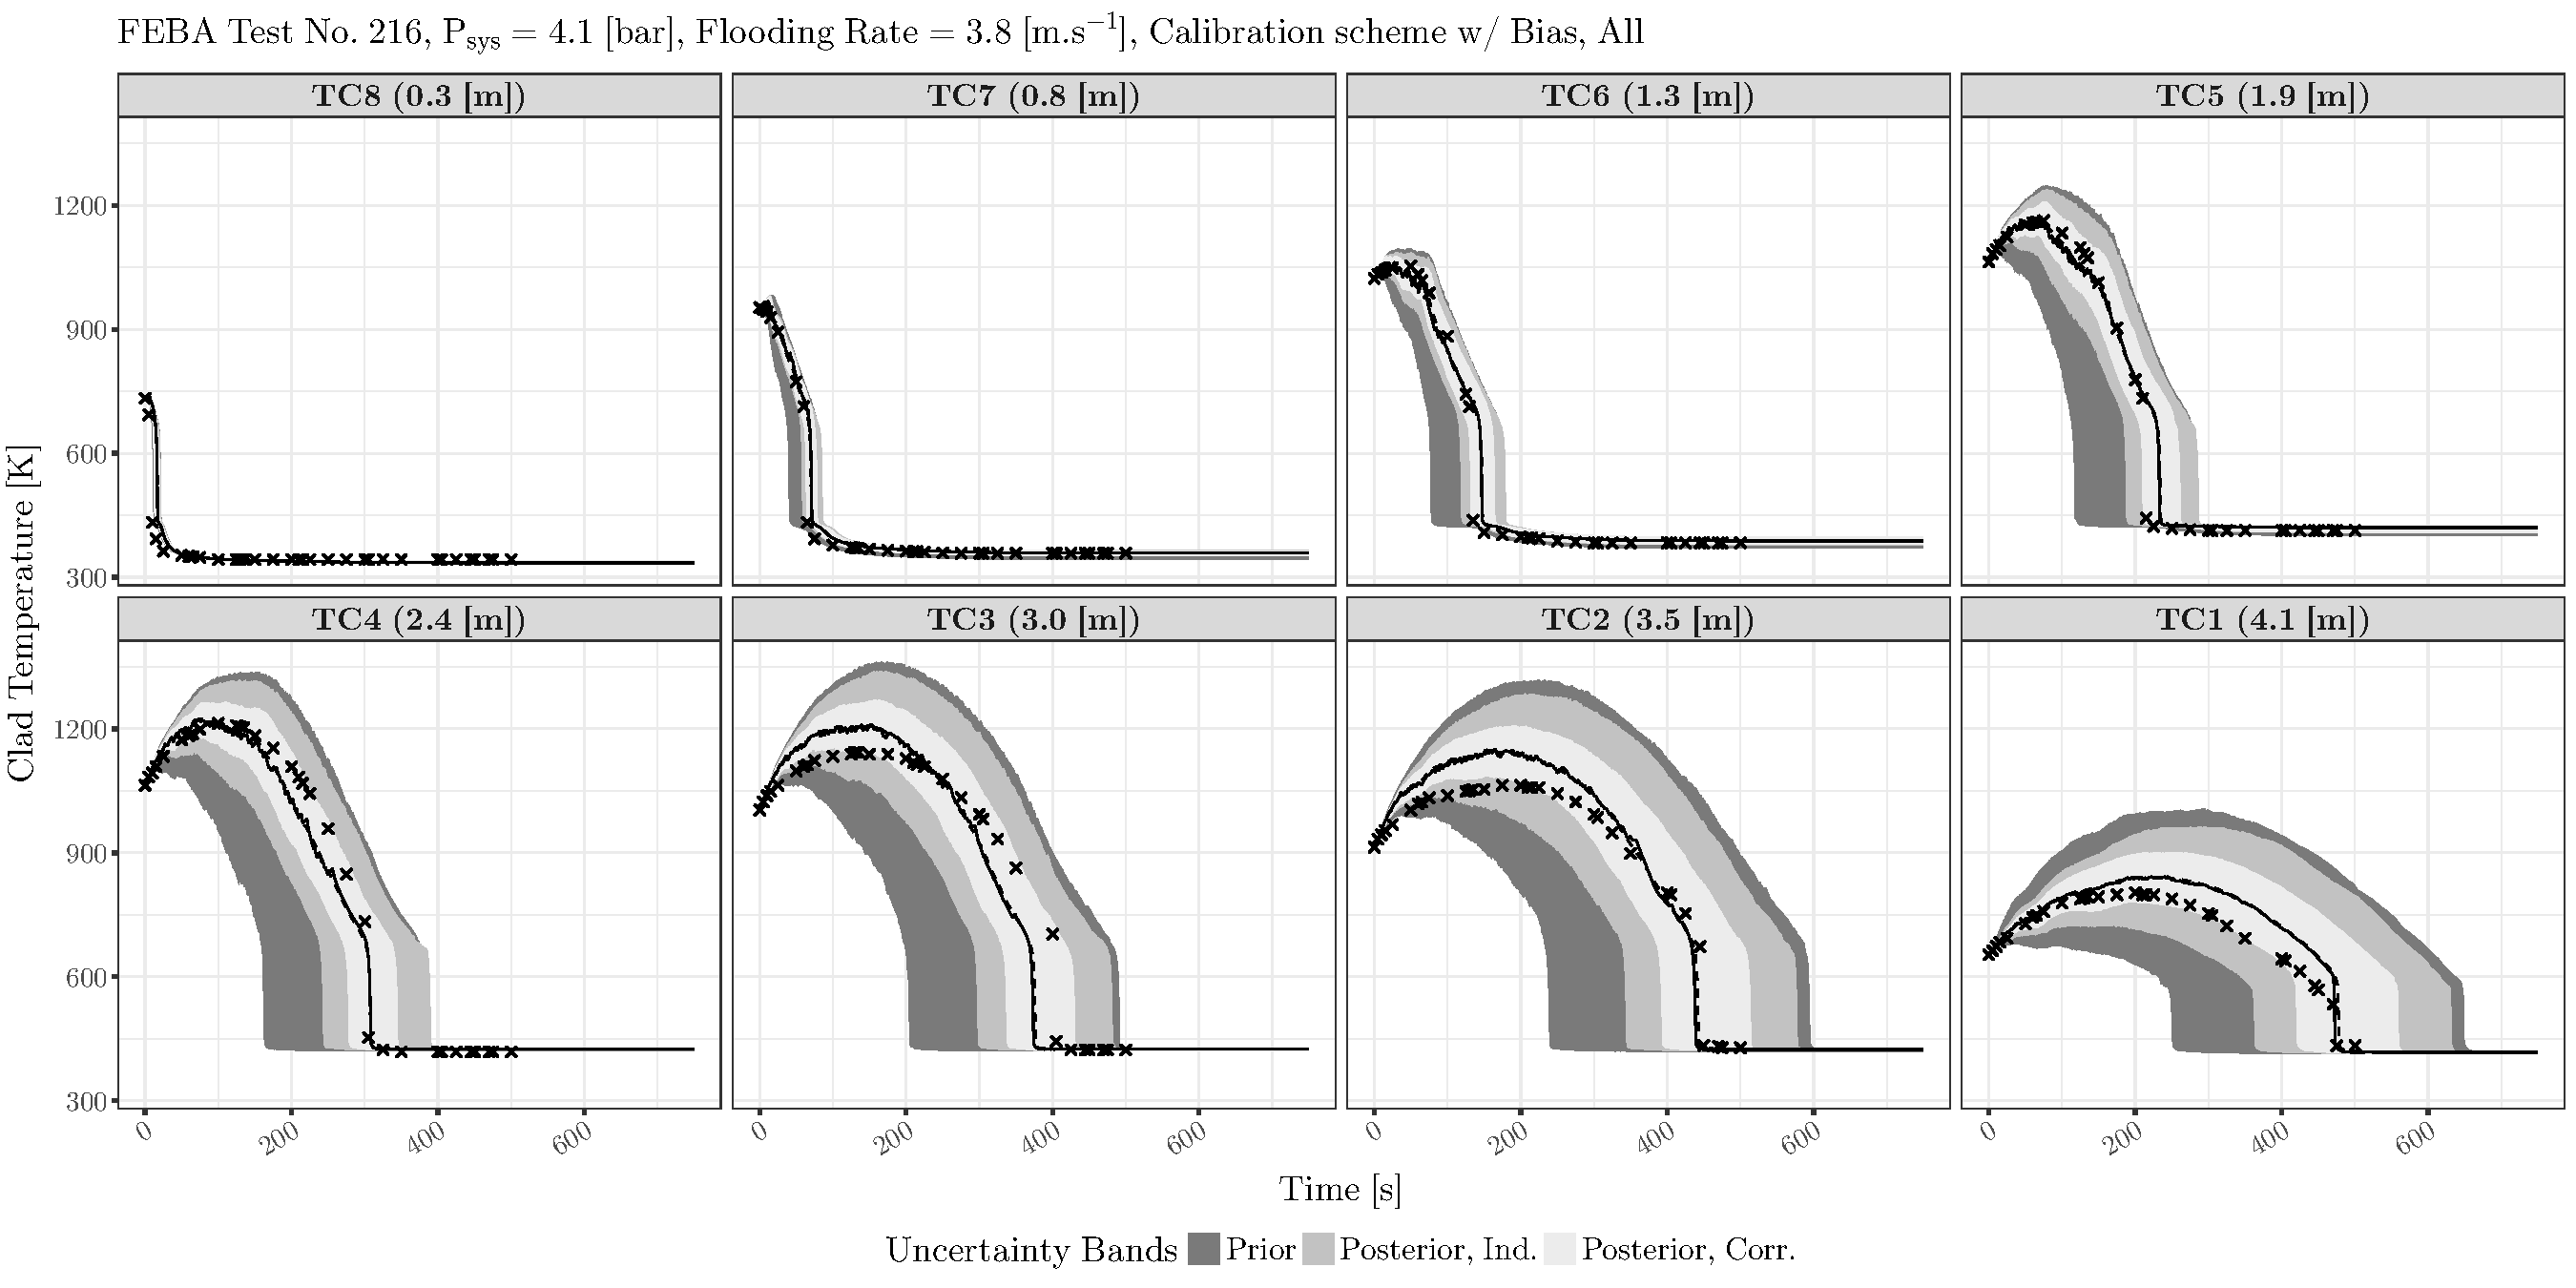
\includegraphics[width=0.90\textwidth]{../figures/chapter5/figures/plotTraceUQPosteriorAllDiscCenteredTC216}
		\captionof{figure}[Propagation of the model parameters uncertainty on FEBA test No. $216$ for the cladding temperature output ($TC$). The posterior samples are from the calibration scheme \texttt{w/ Bias, All}.]{Propagation of the model parameters uncertainty on FEBA test No. $216$ for the cladding temperature output ($TC$) at different axial locations. The uncertainty bands refer to the symmetric $95\%$ probabilities. Solid lines, dashed lines, and crosses indicate the simulation with the nominal parameters values, the median of the posterior, and the experimental data, respectively. The posterior samples are from the calibration with model bias term and considering all types of output (\texttt{w/ Bias, All}).}
	\label{fig:ch5_plot_trace_uq_post_all_disc_tc_216}
\end{sidewaysfigure}

% Explaining the figure, TC
Fig.~\ref{fig:ch5_plot_trace_uq_post_all_disc_tc_216} shows the uncertainty propagation for the time-dependent $TC$ outputs at all axial levels with the posterior samples generated by the calibration scheme \texttt{w/ Bias, All}.
The posterior uncertainties of the clad temperature prediction are narrower as compared to the prior uncertainties across all axial elevations and at all time points.
All uncertainty bands, however, shows similar behavior regarding their inflation going from the bottom part of the assembly to the top of the assembly, and from the start of the transient to the time of quenching.
This is well illustrated by the panel of $TC2$ in Fig.~\ref{fig:ch5_plot_trace_uq_post_all_disc_tc_216} which shows that having the uncertainty band to envelop the experimental data points in the early phase of the transient would require a realization of the reflood curve that increases the discrepancy in the later phase of the transient, especially near the time of quenching.
There is an apparent ``rigidity'' associated with the \gls[hyper=false]{trace} reflood curve which cannot be arbitrarily bend.
Lastly, the median of the posterior predictions (dashed lines) coincides almost perfectly with the prediction of the nominal \gls[hyper=false]{trace} run (solid lines).

% Correlated vs. Independent
Not considering the correlation between model parameters in the posterior samples results in wider uncertainties in the clad temperature prediction.
While the prediction lower uncertainty bound in this case is much narrower than that of the prior, the prediction upper uncertainty bound is closer to the upper uncertainty bound of the prior.
That is, the prediction upper bound is less constrained.

% FEBA Test No. 216 Posterior w/ bias term Uncertainty Propagation, DP
Fig.~\ref{fig:ch5_plot_trace_uq_post_all_disc_dp_216} shows the uncertainty propagation for the time-dependent $DP$ outputs for each of the axial segments.
The posterior samples correspond to the calibration scheme \texttt{w/ Bias, All}.
Once again the posterior uncertainties propagation result in narrower uncertainty bands as compared to that of the prior.
However, the difference between taking and not taking into account correlation between model parameters is less striking for this type of output.
Moreover, all uncertainty bands cover most of the experimental data.
\bigfigure[pos=tbhp,
           opt={width=1.0\textwidth},
           label={fig:ch5_plot_trace_uq_post_all_disc_dp_216},
           shortcaption={Propagation of the model parameters uncertainty on FEBA test No. $216$ for the pressure drop output ($DP$). The posterior samples are from the calibration scheme \texttt{w/ Bias, All}.}]
{../figures/chapter5/figures/plotTraceUQPosteriorAllDiscCenteredDP216}
{Propagation of the model parameters uncertainty on FEBA test No. $216$ for the pressure drop output ($DP$) at different axial segments. The uncertainty bands refer to the symmetric $95\%$ probabilities. Solid lines, dashed lines, and crosses indicate the simulation with the nominal parameters values, the median of the posterior, and the experimental data, respectively. The posterior samples are from the calibration scheme \texttt{w/ Bias, All}.}

% FEBA Test No. 216 Posterior w/ bias term Uncertainty Propagation, CO
Fig.~\ref{fig:ch5_plot_trace_uq_post_all_disc_co_216} shows the propagation for the time-dependent $CO$ output up to the saturation of the measurement tank at $10 [kg]$ with the posterior samples corresponding to the calibration scheme \texttt{w/ Bias, All}.
Unlike the previous two types of output, the nominal \gls[hyper=false]{trace} prediction exhibits a large bias compared to the experimental data.
While the large prior uncertainty manages to cover the experimental data points, all of the points fall outside the posterior uncertainty bounds both with and without taking into account correlation among parameters.
As the calibration scheme \texttt{w/ Bias, All} simultaneously takes into account the three types of output, it can be inferred that this failure to cover the experimental data points is off-set by the more consistent bands for the other two outputs.
\begin{figure}[!bth]
    \centering
    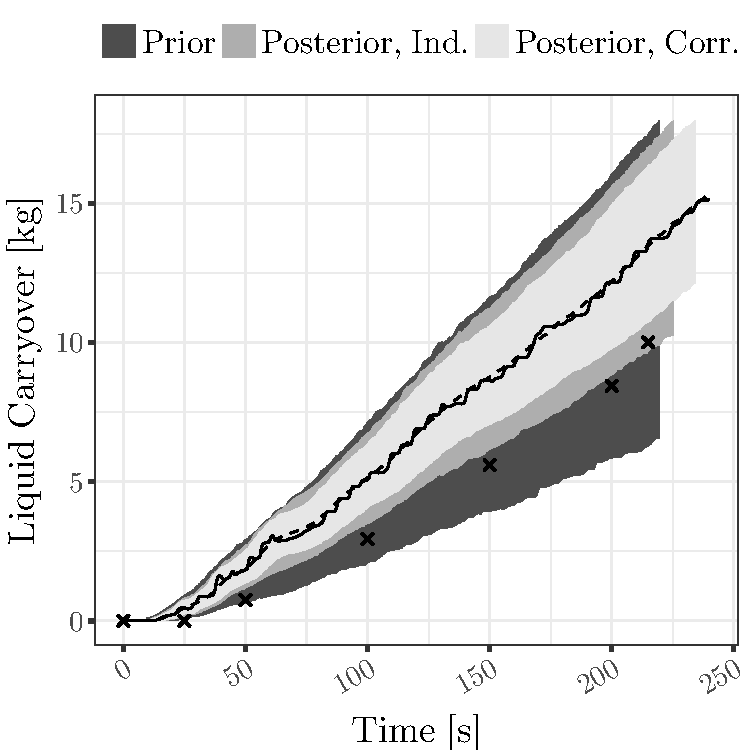
\includegraphics[width=0.5\textwidth]{../figures/chapter5/figures/plotTraceUQPosteriorAllDiscCenteredCO216}
    \caption[Propagation of the model parameters uncertainty on FEBA test No. $216$ for the liquid carryover output ($CO$). The posterior samples are from the calibration scheme \texttt{w/ Bias, All}.]{Propagation of the model parameters uncertainty on FEBA test No. $216$ for the liquid carryover output ($CO$). The uncertainty bands refer to the symmetric $95\%$ probabilities. Solid lines, dashed lines, and crosses indicate the simulation with the nominal parameters values, the median of the posterior, and the experimental data, respectively. The posterior samples are from the calibration scheme \texttt{w/ Bias, All}.}
    \label{fig:ch5_plot_trace_uq_post_all_disc_co_216}
\end{figure}

% Calibration Score vs Informativeness
Similar plots of the propagation of uncertainty of the model parameters generated from all calibration schemes considered on all \gls[hyper=false]{feba} tests are presented in Appendix~\ref{app:mcmc_evaluation}.
Fig.~\ref{fig:ch5_plot_calib_info} is used to summarize the effect of the uncertainty propagation by plotting the \emph{calibration score} vs. \emph{informativeness} (see Section~\ref{subsub:bc_calibration_evaluation}).

% How to read the plot
In each panel, the vertical lines correspond to the informativeness of the prior relative to a rectangular (i.e., representing a state of ignorance) model,
which is $0.5$ uniformly across output types and \gls[hyper=false]{feba} tests.
The horizontal lines correspond to the calibration score of the prior uncertainty bands and the nominal \gls[hyper=false]{trace} run as its reference simulation value.
As can be seen the scores are slightly different from test to test and from output type to output type.
Finally, the results of propagating the posterior samples obtained from each calibration scheme to the \gls[hyper=false]{trace} \gls[hyper=false]{feba} model are plotted.
Increasing the informativeness is equivalent to narrowing the uncertainty band;
while increasing the calibration scores indicates that the prediction and its uncertainty are closer to the experimental data.

% Comparing Results, calibration scheme
For the $TC$ output, and except for \gls[hyper=false]{feba} test No. $216$ (the calibration data), there is an apparent linear relationship between calibration score and informativeness.
That is, the propagation that results in narrower uncertainty band (high informativeness) tends to have a higher failure in enveloping the experimental data (low calibration score)\footnote{Recall that a failure in enveloping experimental data points is assigned to have a zero calibration score.}.
The results of the scheme \texttt{w/o Bias}, in particular, have among the lowest calibration score with respect to the $TC$ output and the highest informativeness. 
On the other hand, for the same level of informativeness, the results of the scheme \texttt{w/ Bias, All} have higher calibration scores across all the \gls[hyper=false]{feba} tests.

This relationship does not hold for the $DP$ output.
There, all the calibration scores fall near the initial calibration score, while having a higher informativeness.
Furthermore, there is less variation in informativeness; the points tend to be clustered together especially in comparison with that of $TC$.

Finally, most calibration schemes result in much lower calibration score with respect to the $CO$ output, some even fall to zero.
That is, the resulting uncertainty bands completely fail to envelop a single experimental data points.
At the same time, the results of the scheme \texttt{w/o Bias} (and with the exception of \gls[hyper=false]{feba} test No. $218$), manage to improve the prediction of the output, both in terms of calibration score and informativeness; the results are better compared to that of the prior.

% Comparing Results, correlated vs independent posterior samples
Considering correlation between the model parameters in the propagation affects the calibration score and the informativeness.
It consistently increases the informativeness (tightening the uncertainty band) and lowers the calibration score across all the \gls[hyper=false]{feba} tests.
The effect can be observed across outputs, calibration schemes, and \gls[hyper=false]{feba} tests; though it is especially strong for the scheme \texttt{w/ Bias, All} and for the $TC$ output.

\begin{sidewaysfigure}
	\centering
	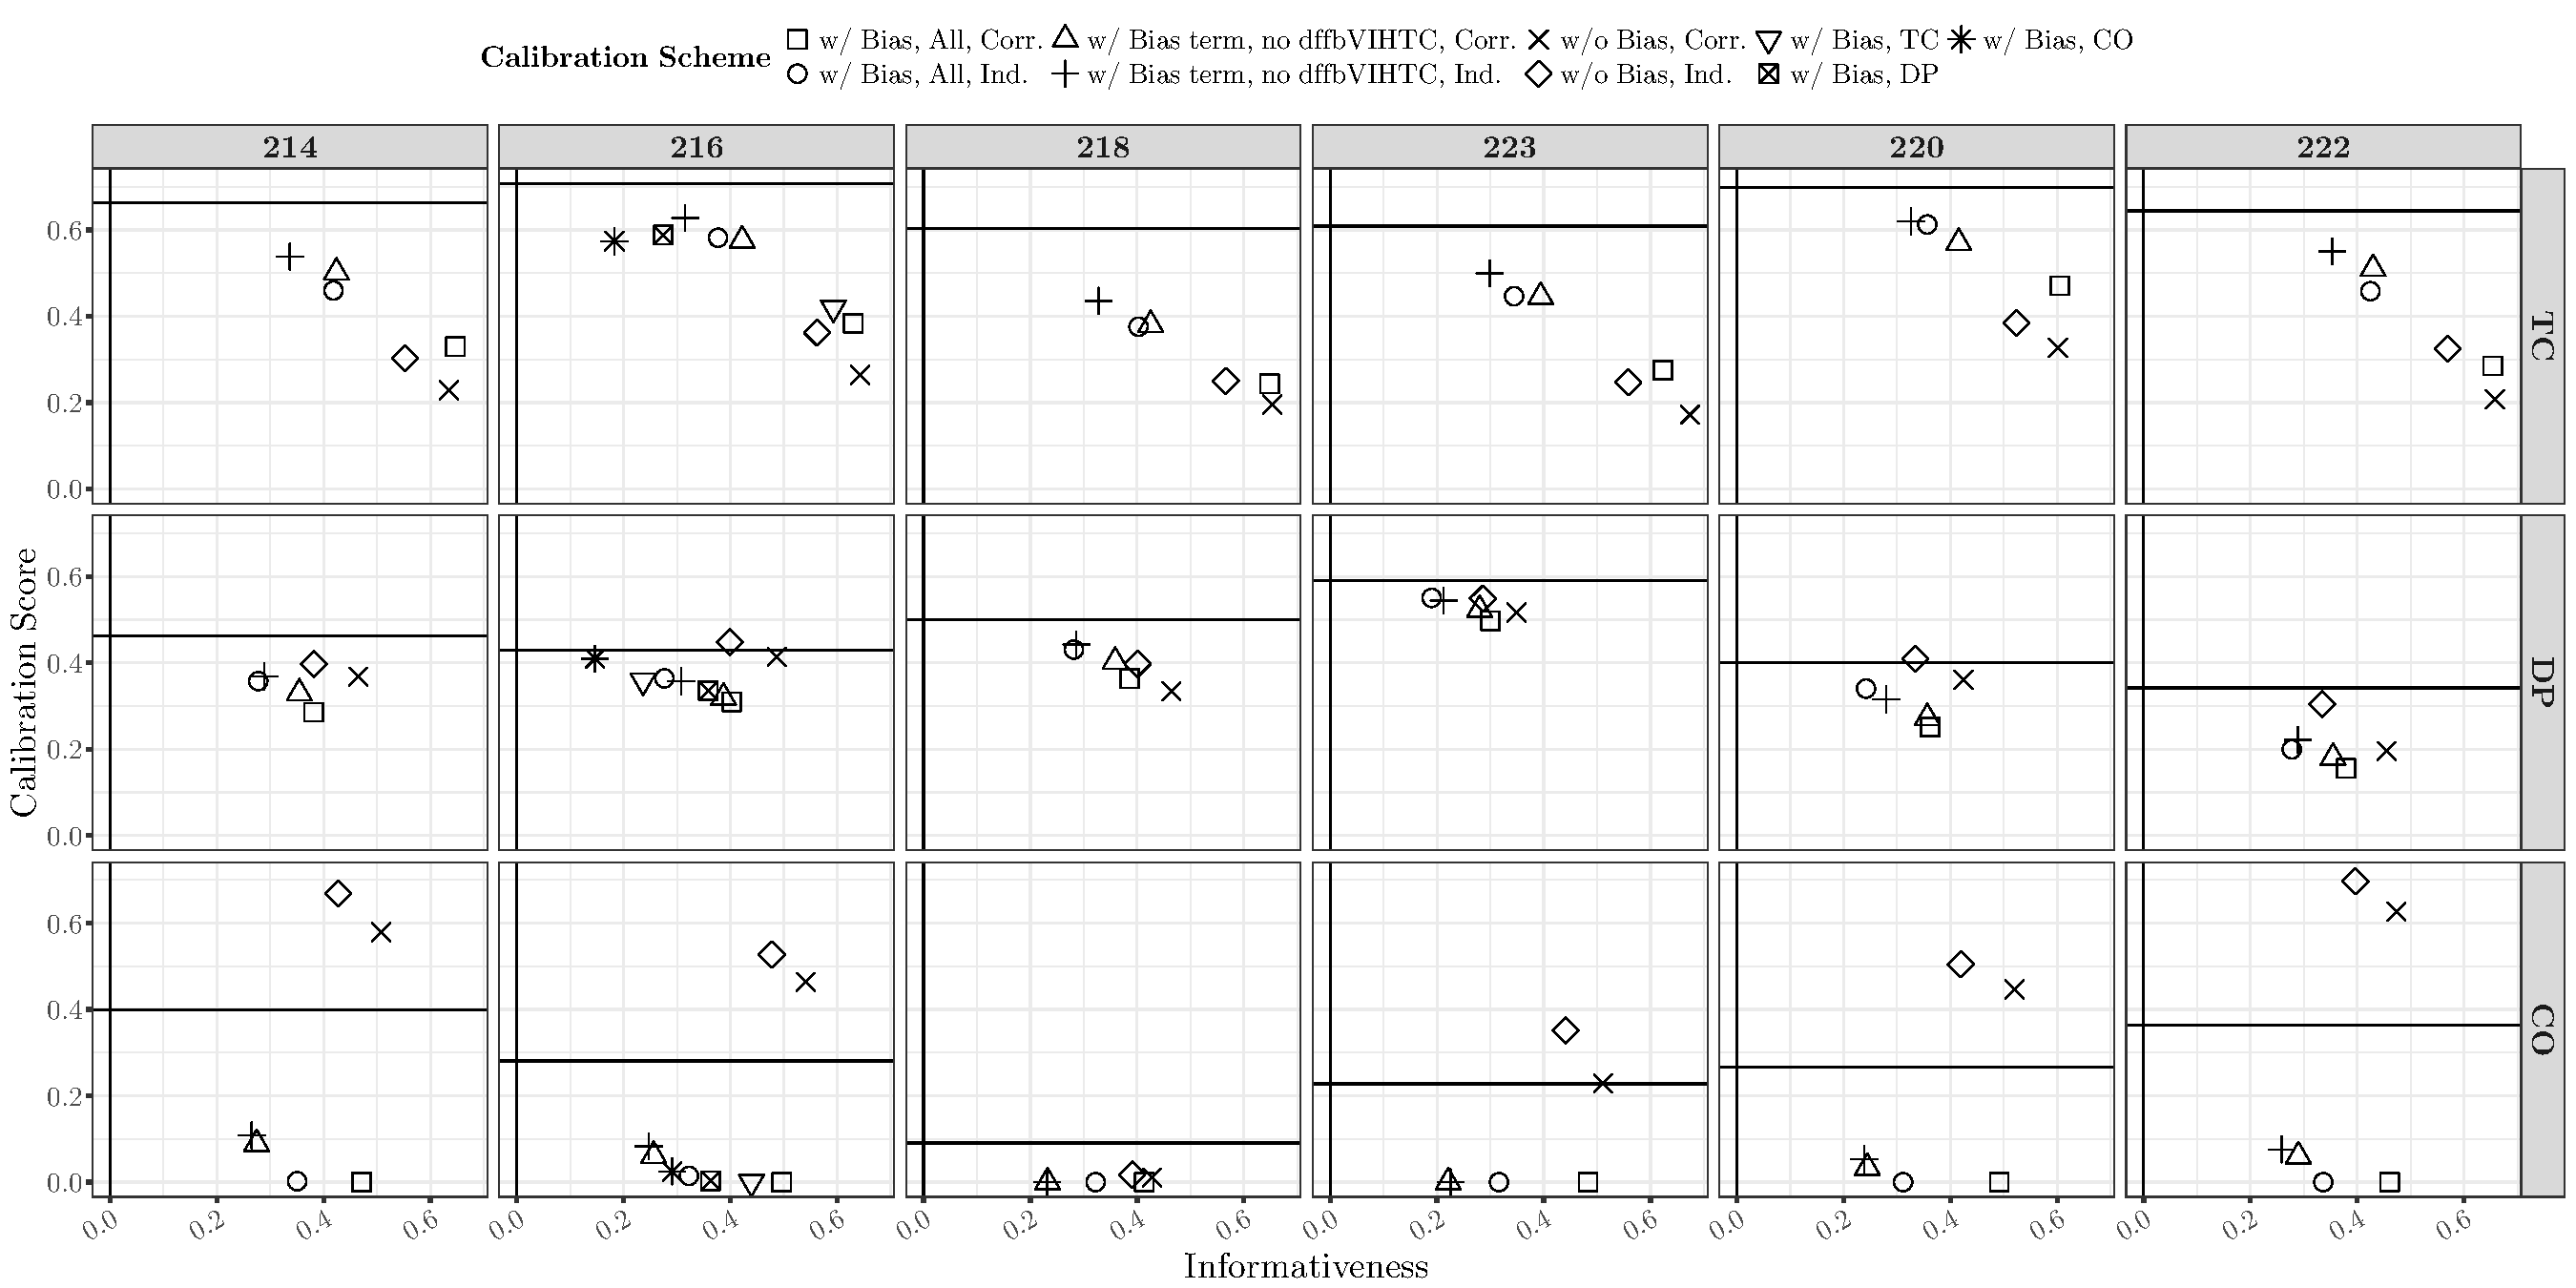
\includegraphics[width=0.95\textwidth]{../figures/chapter5/figures/plotCalibInfo}
		\captionof{figure}[Calibration score vs. Informativeness for different posterior samples propagated on all the FEBA tests.]{Calibration score vs. Informativeness for different posterior samples propagated on all the \gls[hyper=false]{feba} tests. Vertical lines indicate the informativeness of the prior uncertainty (defined as $0$) while the horizontal lines indicate the initial Calibration score (i.e., that of the prior).}
	\label{fig:ch5_plot_calib_info}
\end{sidewaysfigure}

% Comparing Results, between FEBA Tests
Comparing results across \gls[hyper=false]{feba} tests shows that the informativeness and the calibration score of each calibration scheme remain similar.
In particular, the maximum informativeness with respect to the $TC$, $DP$, $CO$ outputs are about $0.7$, $0.5$, $0.5$, respectively, for all the \gls[hyper=false]{feba} tests.
This indicates that the uncertainty band in the prediction due to the posterior uncertainties (obtained on the basis of a single test) are relatively insensitive to the boundary conditions of the tests.

% Comparing results, different output for FEBA Test 216
Lastly, for \gls[hyper=false]{feba} test No. $216$, Fig.~\ref{fig:ch5_plot_calib_info} also shows the results of the calibration schemes with bias where only the $TC$, $DP$, $CO$ outputs were considered separately. 
As expected, these schemes have a lower informativeness than when considering all types of output together.
And using only a particular type of output causes the informativeness with respect to the other outputs to be particularly lower.
Moreover, the increase in informativeness from taking into account multiple types of output is not followed by a large decrease of the calibration score.
This is especially true for the $DP$ (and $TC$) output where the improvement of the informativeness is significant when compared to the results of calibration using experimental data other than the $DP$ output (and $TC$ output, respectively) itself.
This confirms that considering different model parameters is responsible for the improvement with respect to each output type as was previously showed by sensitivity analysis.
